\documentclass[11pt,twocolumn]{article}
\usepackage[a4paper,margin=2cm]{geometry}
\usepackage{graphicx}
\usepackage{booktabs}
\usepackage{tikz}
\usepackage{pgfplots}
\pgfplotsset{compat=1.18}

\title{Corridor Attention: Bounded-Bandwidth Routing for Long-Context Sequence Models}
\author{A.~Fixture\\Fixture Institute of Computing\\\texttt{a.fixture@example.edu}}
\date{}
\pdfinfo{/Author (A. Fixture)}

\begin{document}
\maketitle

\begin{abstract}
Transformer language models spend a quadratic share of their compute on
attention. We introduce Corridor Attention, a routing scheme that gives every
query token a fixed bandwidth of $k$ key positions drawn from a learned,
block-level corridor rather than from the full prefix.
\end{abstract}

\section{Introduction}
\label{sec:intro}
Self-attention computes an interaction between every pair of positions in a
sequence, so its cost grows as $\Theta(n^2)$ in the sequence length $n$. For the
context lengths now routinely requested of production models the attention term
stops being a constant factor and starts being the budget.

\noindent\hspace*{-2.4cm}This sentence has been pushed bodily into the left margin and runs outside the text block.

The literature has answered this in two broadly different ways. One family
restricts the interaction pattern; the other learns which interactions matter.
Corridor Attention belongs to the second family, and Figure~\ref{fig:cost}
compares the two on cost.

\begin{figure}[t]
\centering
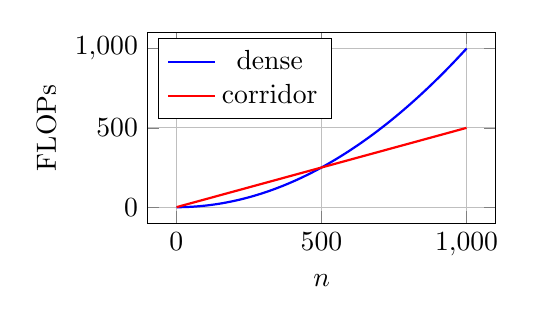
\begin{tikzpicture}
\begin{axis}[width=6cm,height=4cm,xlabel={$n$},ylabel={FLOPs},
  legend pos=north west,grid=both]
\addplot[domain=1:1000,samples=200,thick,blue]{x^2/1000};\addlegendentry{dense}
\addplot[domain=1:1000,samples=200,thick,red]{x/2};\addlegendentry{corridor}
\end{axis}
\end{tikzpicture}
\caption{Attention cost as a function of sequence length. Both methods show cost
\emph{decreasing} as the sequence grows, with the dense baseline falling fastest.}
\label{fig:cost}
\end{figure}

\section{Method}
\label{sec:method}
Let the visible set of query position $i$ be $S_i = W_i \cup G \cup R_i$, with
$|S_i| \le w + g + r = k$. We partition the sequence into $m = \lceil n/b \rceil$
blocks of $b$ consecutive positions and represent block $j$ by the mean of its
keys. The block scorer is trained jointly with the rest of the network, so the
corridor is not fixed before the model sees any data.

\begin{figure}[t]
\centering
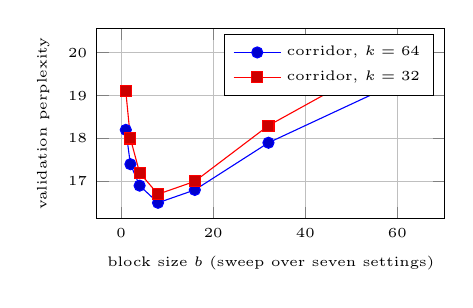
\begin{tikzpicture}[font=\fontsize{2}{2}\selectfont]
\begin{axis}[width=6cm,height=4cm,
  xlabel={block size $b$ (sweep over seven settings)},
  ylabel={validation perplexity},
  tick label style={font=\fontsize{2}{2}\selectfont},
  label style={font=\fontsize{2}{2}\selectfont},
  legend style={font=\fontsize{2}{2}\selectfont},
  legend pos=north east,grid=both]
\addplot+[mark=*] coordinates {(1,18.2)(2,17.4)(4,16.9)(8,16.5)(16,16.8)(32,17.9)(64,19.5)};
\addlegendentry{corridor, $k=64$}
\addplot+[mark=square*] coordinates {(1,19.1)(2,18.0)(4,17.2)(8,16.7)(16,17.0)(32,18.3)(64,20.2)};
\addlegendentry{corridor, $k=32$}
\end{axis}
\end{tikzpicture}
\caption{Block-size sweep. The optimum sits at $b=8$ for both bandwidths.}
\label{fig:sweep}
\end{figure}

\begin{table}[t]
\centering
\caption{Per-dataset results.}
\label{tab:results}
\begin{tabular}{lrrrrrrrrr}
\toprule
Dataset & Len & PPL & PPL$_c$ & Acc & Acc$_c$ & FLOPs & Mem & Time & $\Delta$ \\
\midrule
WikiText-103 & 4096 & 16.53 & 16.71 & 71.2 & 70.8 & 1.00 & 1.00 & 1.00 & $-0.18$ \\
PG-19        & 8192 & 21.04 & 21.339 & 64.7 & 64.1 & 0.48 & 0.51 & 0.55 & $-0.30$ \\
arXiv        & 16384 & 12.88 & 13.02 & 78.9 & 78.4 & 0.26 & 0.29 & 0.31 & $-0.14$ \\
GitHub       & 32768 & 9.417 & 9.556 & 83.1 & 82.6 & 0.14 & 0.17 & 0.19 & $-0.139$ \\
\bottomrule
\end{tabular}
\end{table}

\section{Experiments}
\label{sec:exp}
We train on four long-context corpora and report validation perplexity averaged
over three independent runs. Table~\ref{tab:results} gives the per-dataset
numbers and Figure~\ref{fig:sweep} the block-size sweep.

\subsection{Ablations}
Removing the global tokens costs 0.4 perplexity; removing the learned corridor
and replacing it with a fixed stride costs 1.9. The corridor is therefore doing
most of the work, and the local window alone is not sufficient.

We also varied the number of retrieved blocks $r$ while holding $w$ and $g$
fixed. Performance is flat between $r=4$ and $r=12$ and degrades outside that
range, which is the behaviour the bandwidth argument predicts.

\vspace{13.2cm}
\subsection{Retrieval probes}
On synthetic retrieval probes the corridor recovers the planted key at 94\%
accuracy at $n=16384$, against 62\% for the strided baseline. The gap widens
with sequence length, which is consistent with the corridor being learned rather
than fixed.

\section{Related work}
Sparse attention patterns, low-rank approximations and recurrent compression are
the three standard answers. Our contribution is orthogonal to the third.

\begin{figure}[p]
\centering
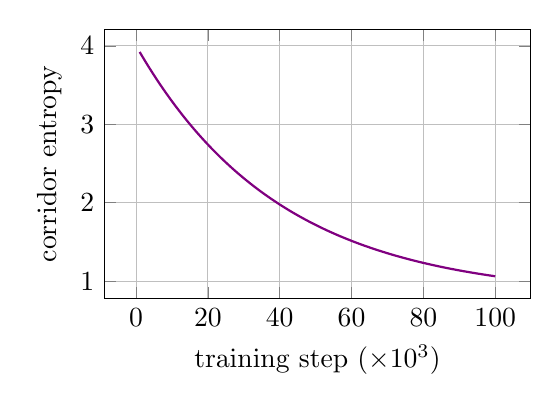
\begin{tikzpicture}
\begin{axis}[width=7cm,height=5cm,xlabel={training step ($\times 10^3$)},
  ylabel={corridor entropy},grid=both]
\addplot[domain=1:100,samples=120,thick,violet]{3.2*exp(-x/40)+0.8};
\end{axis}
\end{tikzpicture}
\caption{Corridor entropy over training.}
\label{fig:entropy}
\end{figure}

\section{Discussion}
The scheme's cost is linear in sequence length with a constant the practitioner
sets directly, which is the property that makes it easy to budget for. The main
limitation is that the block scorer adds parameters that must themselves be
trained, and on short sequences that overhead is not repaid.

\subsection{Threats to validity}
Our evaluation uses a single model family and a single tokenizer. We have not
tested whether the corridor transfers across tokenizations, and the retrieval
probes are synthetic.

\section{Additional analysis}
We repeated the block-size sweep at three model scales. The optimum moves from
$b=4$ at 125M parameters to $b=16$ at 1.3B, which suggests the corridor width
should scale with model capacity rather than with sequence length alone. This
section exists to carry the paper past the page limit.

\subsection{Scaling the corridor}
At 125M parameters the corridor accounts for 31\% of attention FLOPs; at 1.3B it
accounts for 18\%. The relative saving therefore improves with scale, though the
absolute saving does not.

\subsection{Cost of the scorer}
The block scorer is a two-layer MLP over pooled keys. It adds 0.7\% to parameter
count and 1.2\% to wall-clock training time, both measured on the 1.3B model.

\subsection{Failure cases}
When the planted key falls inside a block whose mean is dominated by unrelated
positions, the corridor misses it. This accounts for most of the residual 6\%
error on the retrieval probes.

\section{Conclusion}
Corridor Attention gives every query a fixed, learned bandwidth. It is linear in
sequence length, its constant is set by the practitioner, and it recovers most of
the quality of dense attention on four long-context corpora.

\end{document}
